\chapter{Success of Markdown, and its divergent paths}
\label{chap:proliferation}

\vspace{1cm}

As seen in chapter \ref{chap:issues}, the qualities of Markdown outweighing its flaws, and opinionated people wanting to solve its issues
their own way, the proliferation of new syntaxes and interpreters that are supersets or modifications of the original syntax made their appearance,
which are commonly called ``markdown flavours''. These allowed many tools and use-cases to come to life, which go far beyond than simple document
markup.

\section{One syntax, many implementations}

The will of the people to "fix" Markdown led to dozens of implementations of it existing in the wild. All of these take opinionated stances
about how to fix the issues found in the language, or augment its feature set. Of course like most divergent standards tend to do, most of them
disagree on how and what to fix, or implement different features. The lack of a proper Markdown standard specification led to dozens of
it now existing.\newline

Indeed, even extremely simple examples of Markdown documents lead to many different HTML outputs depending on the type of implementation used
to interpret the markdown snippet. In order to visualise the absurdity of it all, \citeauthor{babelmark} created a tool called
"Babelmark"\footcite{babelmark} (named after the Tower of Babel origin myth and the ``confusion of languages'' that supposedly happened there)
which allows to take a Markdown document and list all known HTML outputs one would have with all the tools available online.
On figure \ref{fig:babelmark}, we see a simple example of a markdown text: two headings of level 1 and 2, with no other text.
Even this short document leads to six different HTML outputs (three of which are shown in the figure).

\begin{figure}[H]
\centering
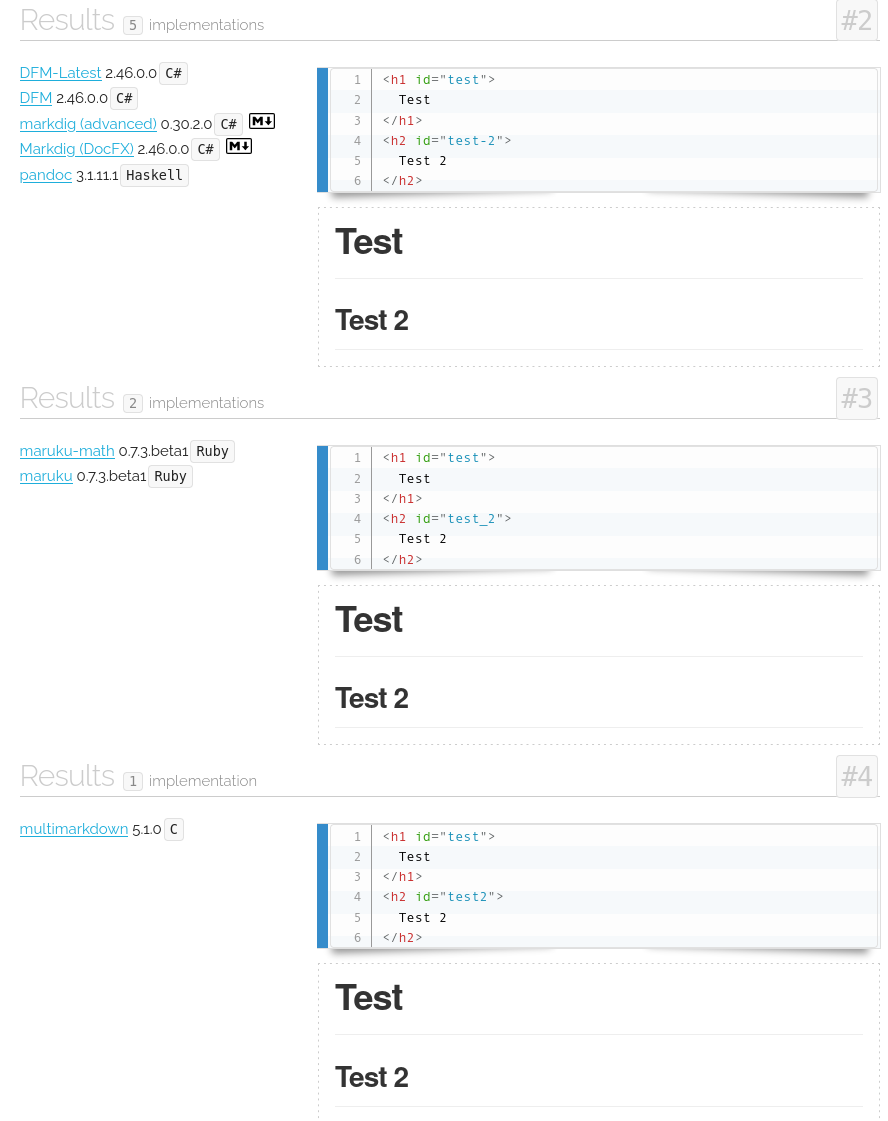
\includegraphics[scale=0.35]{babelmark}
\caption{Babelmark listing many possible outputs from markdown implementations}
\label{fig:babelmark}
\end{figure}

This lack of common ground led a group of people to push for a standard specification of Markdown to be created.

\section{Standardization efforts}

xx \footcite{leonard2016text}

xx \footcite{commonmark}

\section{Markdown ``flavours'', extensions and their impacts}

% TODO:
% Discuss Github flavored markdown, Obsidian, MKDocs, etc

xx \footcite{voegler2014markdown}